% Chapter 1

\chapter{Some Basic Simulations} % Main chapter title

\label{Chapter1} % For referencing the chapter elsewhere, use \ref{Chapter1} 

\lhead{Chapter 1. \emph{Chapter Title Here}} % This is for the header on each page - perhaps a shortened title

%----------------------------------------------------------------------------------------


While the introduction outlined the computer programming necessary to produce simulations in general, this chapter will start to deal with the physics necessary to make simulations seem realistic.  In this chapter, I will outline some examples of simulations with balls bouncing, and discussing the basic mechanics involved through the code.



\section{Basic Ball Bouncing}

A ball bouncing will show the basic kinematic equations, and how they are used in the javascript code.  The following example displays a ball being dropped with an initial $v_x$, and bouncing off the walls and floor of the canvas element.  The full code is shown below:




\setstretch{1}
\begin{lstlisting}[breaklines=true, frame=single, numbers=left, caption=A basic ball bouncing simulation, label=lst:basicballbounce]
var canvas = document.getElementById(`canvas');
var context = canvas.getContext(`2d'); 

canvas.height = screen.height-200;
canvas.width = screen.width -100;

var radius = 20;
var color = ``red";
var g = .1635; // acceleration due to gravity
var x = 40;  // initial horizontal position
var y = 40;  // initial vertical position
var vx = parseFloat(prompt(`what is the initial horizontal speed of ball you would like?(recommended values of 1-20'));  // initial horizontal speed 
var vy = 0;  // initial vertical speed
 
window.onload = init; 
 
function init() {
  setInterval(onEachStep, 1000/60); // 60 fps
};
 
function onEachStep() {
  vy += g; // gravity increases the vertical speed
  x += vx; // horizontal speed increases horizontal position 
  y += vy; // vertical speed increases vertical position

  if (y > canvas.height - radius){ // if ball hits the ground
    y = canvas.height - radius; // reposition it at the ground
    vy *= -0.8; // then reverse and reduce its vertical speed
  }
  if (x > canvas.width - radius){ // if ball hits right wall
    x = canvas.width - radius; // reposition it right at wall 
    vx *= -0.8;  // then reduce and reverse horizontal speed
  }
  if (x < radius){  // if ball hits left wall
    x = radius;  // reposition it right at wall
    vx *= -0.8  // then reverse and reduce horizontal speed
  }
  drawBall(); // draw the ball
};
 
function drawBall() {
  with (context){
    clearRect(0, 0, canvas.width, canvas.height); 
    fillStyle = color;
    beginPath();
    arc(x, y, radius, 0, 2*Math.PI, true);
    closePath();
    fill();
  };
};

\end{lstlisting}
\setstretch{2}

This code functions by first setting up the canvas to be an appropriate size, on lines 1-5.  Then, the simple variables of radius, color, initial positions/velocities, and acceleration are initialized.  As mentioned in the introduction, the canvas HTML element defines positions in terms of pixels, with the top left corner of the canvas being the origin.  Therefore, the ball is initialized to appear at (40, 40) which is near the top left corner for any computer screen.  The value of g, the gravitational constant, is set to .1635 to accurately represent its value near Earth's surface, of $9.81 \hspace{1mm} \frac{m}{s^2}$.  To understand why this value makes sense, it is necessary to understand the units of velocity on the HTML canvas.  The position during the simulation is given in terms of pixels, which of course differs from the SI unit of meters.  However, as long as g can be initialized to be $9.81 \hspace{1mm} \frac{px}{s^2}$, the simulation will still look physically accurate.  This can be explained with the equation below:

\begin{equation} \label{eq:pixelsconversion}
9.81 \hspace{1mm}  \frac{px}{s^2}  = .1635 \hspace{1mm}  \frac{\frac{px}{s}}{frame} \hspace{1mm}  \times \hspace{1mm}  \hspace{1mm}  \frac{60 frame}{s}
\end{equation}


The value of g is calculated based on the fact that the simulation was run at 60 frames per second.  Time is a central component of all physics, and for the simulations to behave realistically they must carefully take that into account.  

The remainder of the code involves 3 functions that call one another to create the flow of the simulation.  The first function, init (``initialize'') is called when the browser window is loaded(line 15).  This function simply delays the next function, onEachStep, by 16.66 ms, meaning that the function essentially runs 60 times per second, producing the desired 60 frames per second.  Line 18 accomplishes this in a crude method: simulations later will involve more sophisticated techniques.  The onEachStep function contains the instructions for each frame of the simulation.  It involves multiple conditional if-statement loops that create the illusion that the ball bounces off of the walls and floor.  

All 3 conditional loops involve a coefficient of restitution, or $C_r$.  This is a mechanical property, representing how ``bouncy'' the ball is, and measures the ratio of the kinetic energy after and before the impact.  This is derived below:

\begin{equation}\label{eq:cr}
C_r = \sqrt{\frac{KE_f}{KE_i}} = \sqrt{\frac{\frac{1}{2} mv_f^2}{\frac{1}{2} mv_i^2}} = \frac{v_f}{v_i}
\end{equation}

A $C_r$ value of .8 was used for this simulation, which is comparable to that of a tennis ball\textsuperscript{\cite{tennisball}}.  The variable Cr represents this value in the code, and is simply multiplied by the velocity before impact, so the following equation results:

\begin{equation}\label{eq:velocitycr}
v_f = v_i * C_r
\end{equation}

An essential part of any physics simulation involves \textit{collision detection}.  For the simple bouncing ball simulation, this is accomplished by conditional loops for if the ball's position exceeds the canvas constraints.  


The last function of the program, drawBall, simply contains commands for the canvas API to draw.  While these commands can be very complicated and intricate to create the exact visual aesthetic desired, the extent of these commands is not the purpose of this thesis.  Basically, this function works by ``erasing'' the canvas of any previous graphics, and then creating a new visual with the arc() method.   

The logic of the program can be summarized through the flow chart below:


\begin{figure}[h] 
	\centering
		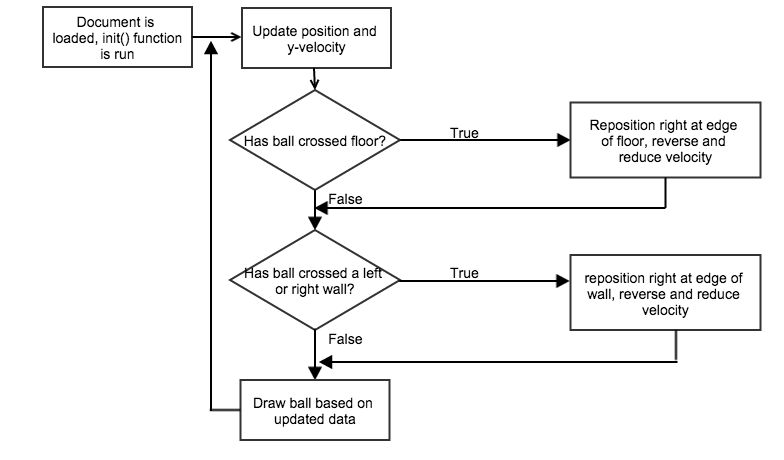
\includegraphics[width=15cm]{Figures/basicbouncingball.png}

	\caption{The logic flow chart of the basic bouncing ball simulation}
	\label{fig:basicbouncingball}
\end{figure}



























